\newif\ifdebug
%\debugtrue
\ifdebug
\documentclass[12pt,a4paper]{ctexrep}
\usepackage[a4paper, portrait, margin=0.8in]{geometry}
\usepackage{graphicx} % Required for inserting images
\usepackage{amsmath}
\usepackage{amsfonts}
\usepackage{amssymb}
\usepackage{amsthm}
\usepackage{markdown}
%\usepackage{china2e} 
\usepackage[utf8]{inputenc}
\usepackage[colorlinks,linkcolor=blue]{hyperref}
\begin{document}
\fi

\chapter{Counting计数, 组合}
Counting, Permutations, Combinations, Balls and Walls, Principle of Inclusion and Exclusion, Generalized Principle of Inclusion and Exclusion, Pigeonhole Principle
\section{定义}
\subsection{Definition of 名词}
Permutations: 排列. [n] = $\{1,2,\dots,n\}$\\$\indent$
Onto:单射.\\$\indent$
\section{定理/结论}
\subsection{几何意义}
[n] has $2^{n}$ subsets\\$\indent$
$\binom{n}{0} + \binom{n}{1} + \binom{n}{2} + \dots + \binom{n}{n} = 2^{n}$\\$\indent$
$\sum_{i=0}^{n} (-1)^{n} \binom{n}{i} = 0$ $\Leftarrow$ even sized subsets=odd sized subsets\\$\indent$
$n \binom{n-1}{k} = (k+1) \binom{n}{k+1}$ $\Leftarrow$ want to choose k+1 people from n people and designate a captain\\$\indent$
$\star \binom{n}{r} = \binom{n-1}{r}+\binom{n-1}{r-1}$ $\Leftarrow$ number of subsets with an arbitrary element + without the element\\$\indent$
$\sum_{0\leq j\leq i\leq n} \binom{n}{i}\binom{i}{j} = 3^{n}$ $\Leftarrow$ separate n into 3 parts\\$\indent$
$\binom{n}{r} = \binom{n}{n-r}$
\subsection{结论}
for [n], how many permutations $\pi$ have the property $\forall i, \pi[i] \neq i$ : $d_{n} = (d_{n-1}+d_{n-2})(n-1)$
\subsection{PIE}
Principle of inclusion and exclusion(PIE): Find the whole number of elements in $A_{1} \sim A_{n}$. \\$\indent$
Generalized PIE: Find the number of elements $E(m)$ appearing in exactly $m$ of $A_{1} \sim A_{n}$. \\$\indent$
$\star$经典习题:6 persons, every pair is either friends or enemy.$\Rightarrow$There must exist 3 people who are friends to each other or enemies to each other.
\section{重要定理详解}
\noindent PIE:\\$\indent$
Let $A_{1}, A_{2}, \dots , A_{n}$ be finite sets.\\$\indent$
Suppose $x$ is in exactly $r$ of the $n$ sets.\\$\indent$
This indicates that $x$ is counted in $\binom{r}{1} \, A_{n}$ s, $\binom{r}{2} \, A_{n_{1}}\cap A_{n_{2}}$ s,$\dots$, $\binom{r}{r} \, A_{n_{1}}\cap A_{n_{2}} \cap \dots \cap A_{n_{r}}$ s.\\$\indent$
$\because$ $-\binom{r}{0}+\binom{r}{1}-\binom{r}{2}+\dots+(-1)^{r+1}\binom{r}{r} +\binom{r}{0}= $ number of subsets with odd sizes - number of subsets with even sizes+1 = 1 \\$\indent$
$\therefore$Set $\omega(t) = \sum_{i_{1},i_{2},\dots,i_{t}}|A_{i_{1}} \cap A_{i_{2}} \cap \dots \cap A_{i_{t}}|$\\$\indent$
$\therefore$ $|\cup_{i=1}^{k} A_{i}| = \sum_{t=1}^{k} (-1)^{t+1} \omega(t)$\\$\indent$
重点在于找$A_{1},A_{2},\dots,A_{n}$!!!\\

\begin{center}
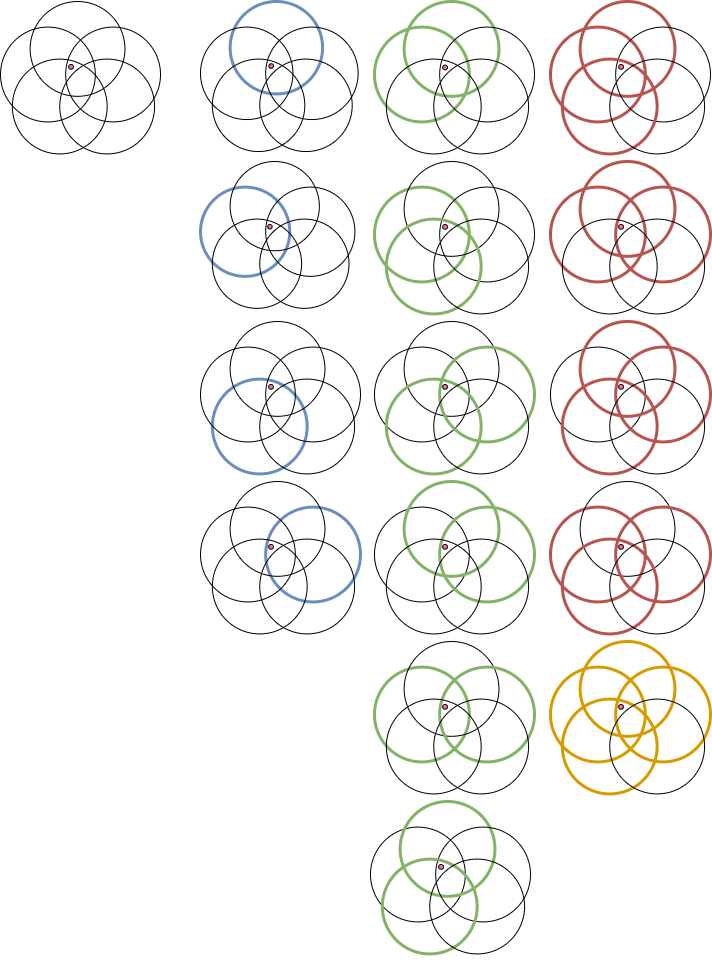
\includegraphics[scale=0.35]{PIE.png}
\end{center}

\noindent Generalized PIE:\\$\indent$
in a universe with n elements, $A_{1}, A_{2}, \dots , A_{n}$ are finite sets\\$\indent$
$\omega(t) = \sum_{i_{1},i_{2},\dots,i_{t}}|A_{i_{1}} \cap A_{i_{2}} \cap \dots \cap A_{i_{t}}|$\\$\indent$
$E(m)$ = the number of elements appearing in exactly $m$ of $A_{1} \sim A_{n}$ = $\sum_{k=m}^{n} (-1)^{k-m} \binom{k}{m} \omega(k)$

An example are as follows:  \href{https://www.youtube.com/watch?v=D1T3xy_vtxU}{vid}

\begin{center}
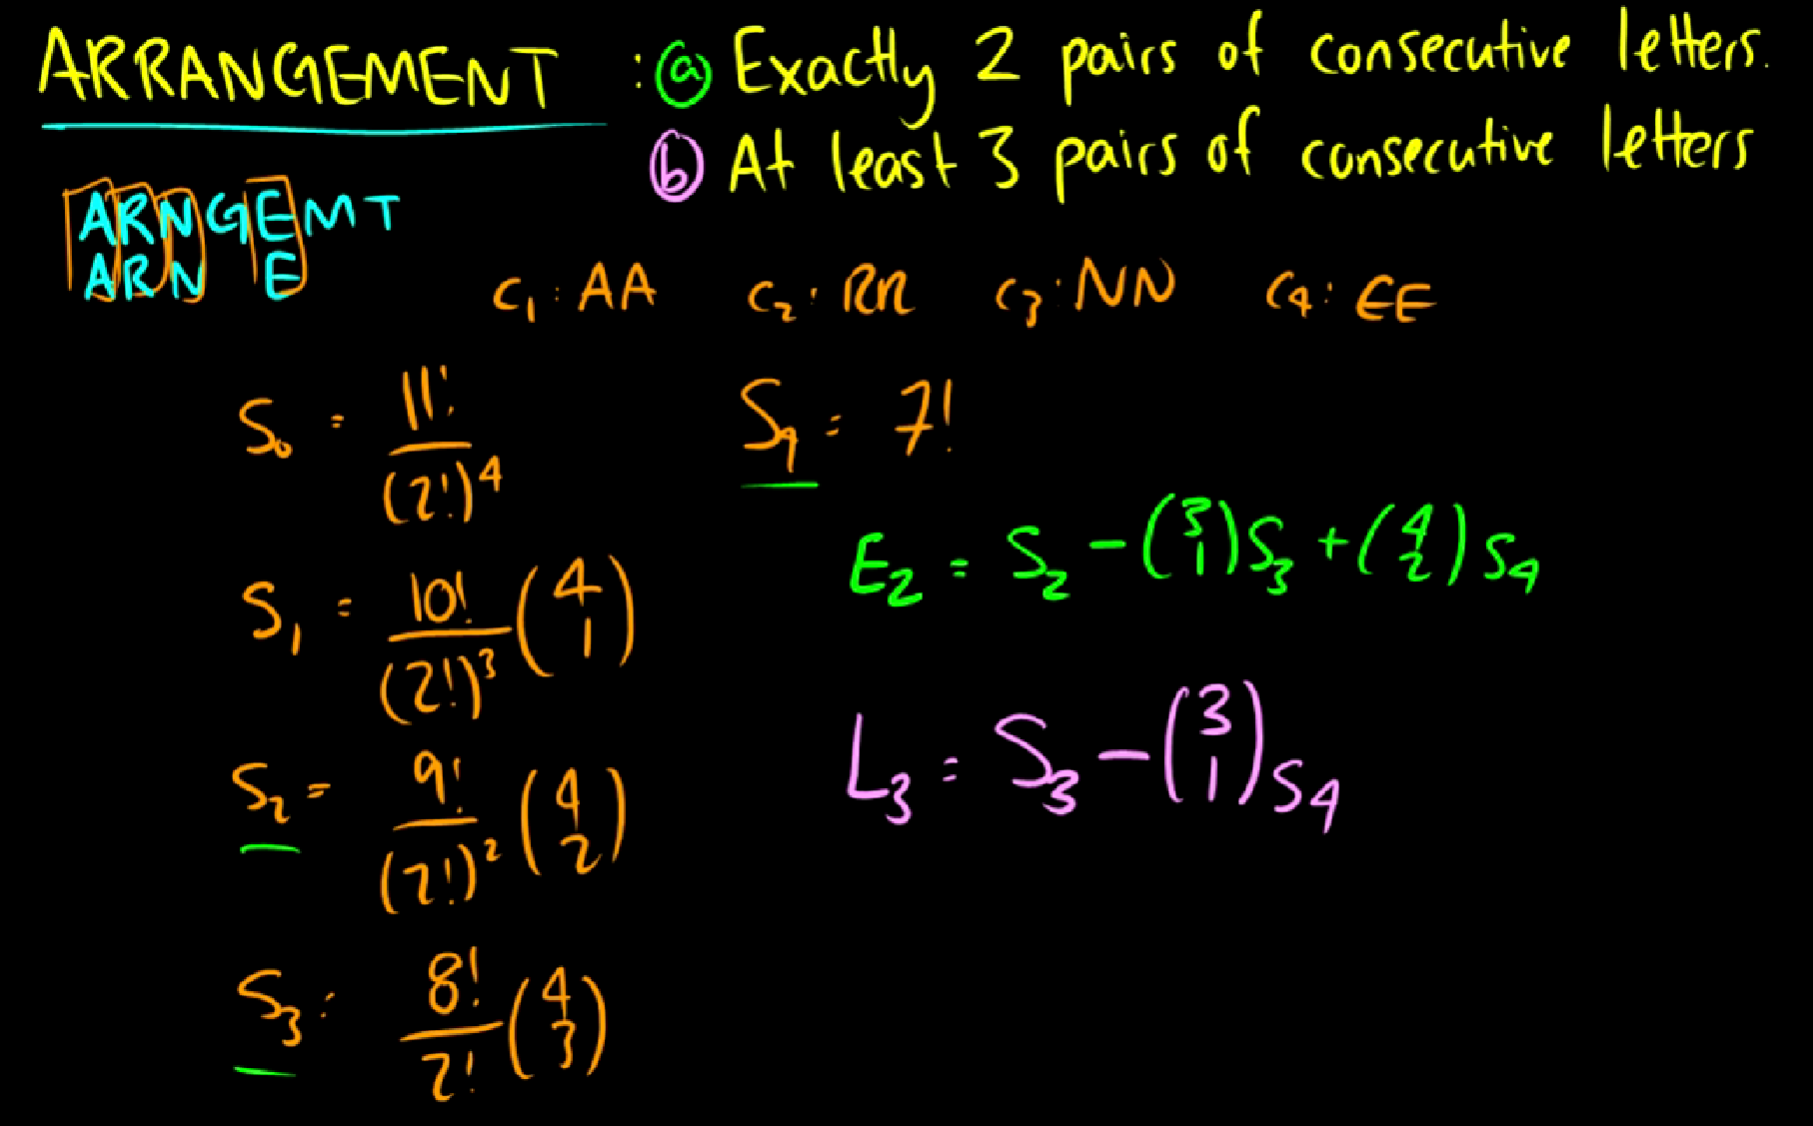
\includegraphics[scale=0.3]{PIE_Example.png}
\end{center}

\section{方法}
Principle of Addition (Case work principle)\\$\indent$
Principle of Multiplication\\$\indent$
算排列的时候别忘了去重\\$\indent$
合理使用induction\\$\indent$
插板法\\

$\indent$题目较长的时候,要么用Pigeon-Hole Principle,要么用induction/strong induction

\ifdebug
\end{document}
\fi